\documentclass[conference]{IEEEtran}
\usepackage{cite}
\usepackage[dvips]{graphicx}
\graphicspath{{./eps/}}
\DeclareGraphicsExtensions{.eps}
\usepackage{amsmath,amssymb,color}
\interdisplaylinepenalty=2500
\usepackage{algorithm}
\usepackage{algorithmic}
\usepackage[table,xcdraw]{xcolor}
\usepackage{array}
\usepackage{mdwmath}
\usepackage{mdwtab}
\usepackage{eqparbox}
\usepackage{multirow}
\usepackage{verbatim}
\usepackage[tight,footnotesize]{subfigure}
%\usepackage{fixltx2e}
\usepackage{url}
\usepackage{balance}
%\setlength{\textfloatsep}{0pt}
%\def\IEEEbibitemsep{0pt plus .5pt}
\IEEEoverridecommandlockouts
\IEEEpubid{\makebox[\columnwidth]{978-1-5386-4649-6/18/\$31.00~\copyright{}2018 IEEE \hfill}\hspace{\columnsep}\makebox[\columnwidth]{ }}

\begin{document}
	
	%================================================================%
	%							                TITLE
	%================================================================%
	%
	\title
	{
	Anomaly Detection in Traffic Flow Data Via Supervised Learning
	}
	
%
%================================================================%
%							                AUTHORS
%================================================================%
%
\author
{
	\IEEEauthorblockN
	{
		Watson Jia\IEEEauthorrefmark{1}
	}
	\IEEEauthorblockA
	{
		Princeton University \\ 
		Email:                                          %
	    \IEEEauthorrefmark{1}watsonj@princeton.edu  %
	}
	\and
	\IEEEauthorblockN
	{
		Raj Mani Shukla\IEEEauthorrefmark{2}
	}
	\IEEEauthorblockA
	{
		University of Nevada, Reno \\
		Email:
		\IEEEauthorrefmark{2}rshukla@unr.edu
	}
	\and
	\IEEEauthorblockN
	{
		Shamik Sengupta\IEEEauthorrefmark{3}
	}
	\IEEEauthorblockA
	{
		University of Nevada, Reno \\
		Email:
		\IEEEauthorrefmark{3}ssengupta@unr.edu
	}
}
%
	
\maketitle



\begin{abstract}
	      The presence of outliers within time series data can have a detrimental effect on the efficiency of automated decision-making applications. In the context of traffic flow, various services reliant on traffic data may be negatively impacted by anomalies due to their dependence on statistical methods. This paper presents an automated anomaly detection algorithm based on supervised learning. The proposed algorithm relies on segmentation and tunable parameters applied to statistical methods to identify outliers in traffic flow data. We measure the efficacy of our algorithm in terms of Precision, Recall, and F-measure from three different perspectives: variation in tunable parameters, outlier magnitude, and outlier prevalence.
\end{abstract}
%\begin{IEEEkeywords}
%Software-defined networks, Plugged-in electric vehicles, Smart grid, Electric vehicle supply equipment 
%\end{IEEEkeywords}
	
	%
	%================================================================%
	%                        INTRODUCTION
	%================================================================%
	%	
\section{Introduction}

The expansion of the Internet of Things (IoT) has enabled a society that has become much more integrated with technology than in the past. Sensors have played an integral role in enabling the growth of IoT and have enabled numerous technological applications in various fields. Through an Internet connection, remotely controlled sensors can gather large amounts of valuable information from the environment and organize the collected data in a central location for analysis. One application is in traffic flow, where sensors can collect traffic information from roads in the form of a time series. By taking advantage of patterns and periodic behavior in these time series, there are many potential applications, such as helping provide for better traffic management by authorities or travel decisions by a commuter \cite{ShuklaVehicleIOT}. Sensors have many other applications such as in smart homes or enabling smart grids, and the effectiveness of these applications can have many benefits for individuals as well as society at large.

However, the data collected by sensors is non-deterministic and can be affected by outside factors. This leads to the presence of outliers within these time series data, which can have an adverse effect on the effectiveness of automated decision-making IoT applications, especially if they are reliant on statistical methods \cite{Hochenbaum2017}. Outliers can be caused by a variety of factors. One source is external environmental factors; for example, in the case of traffic flow, a car accident could lead to an unusual dip in traffic detected by sensors at a given location. In time series data, this may be manifested as a sudden drop in traffic flow for a location. Another source can be the quality of the sensor itself; if the sensor is not properly calibrated or physically tampered with, a given sensor will not be able to collect accurate information. Outliers can be malicious; in a data falsification attack, a malicious actor targets a sensor or a group of sensors and intentionally modifies the data values collected \cite{Vempaty2013}. This is an area of major concern in the IoT, since malicious outliers can negatively impact the effectiveness of decision-making capabilities in IoT-enabled applications. An attacker can directly change the data collected by sensors and impact the effectiveness of data analysis applications. Outliers negatively impact automated statistical analysis in IoT applications. For example, a taxi service may be negatively impacted if it is using data that has been corrupted or otherwise of bad quality.  Thus, it is of great interest that we be able to detect anomalies within time-series data to ensure the effectiveness of data analysis applications. We explore the problem of anomaly detection in time series data from the perspective of traffic flow data collected from sensors throughout the state of California. 

The problem of anomaly detection presents several challenges. For one, there are a myriad of sensors connected to the IoT, each of which can collect a wide variety of data. Moreover, in the context of our problem, different traffic flow sensors have different challenges that must be addressed. For example, some sensors are located remotely and experience adverse conditions in comparison to sensors located in urban areas. Due to the sheer quantity of data that must be considered as well as challenges with each individual sensor, manual outlier detection is infeasible. Automated statistical analysis must be conducted instead to be able to process these large amounts of data quickly and identify outliers within them. This suggests a supervised learning approach, however, there is a lack of labeled outlier data to be able to train learning models for this problem. Moreover, there is the question of what statistical methods and tests may be effective in outlier detection – that is, what statistical metrics may be robust to outlier influences so that they can identify outliers with a high degree of accuracy.

There are multiple statistical properties that time series data can exhibit, such as mean, median, and M-estimator. These properties are often used in statistical outlier detection tests, each with their own advantages and disadvantages. The mean can be accurate in describing the central tendencies of normally distributed data sets as well as skewed distributions such as log-normal and Poisson distributions. However, the mean is not a robust statistic and is heavily influenced by the presence of outliers. In contrast, the median is a robust measure of central tendency but may not be as accurate in describing the central tendencies of skewed distributions. M-estimators have the benefits of being robust as well as being able to provide a sample average. However, computing M-estimators is more complex and involved. In this paper we combine these three statistical properties of the data samples to detect outliers. Furthermore, once outliers are present in data, the robust statistical measures may not deviate but the minimum and maximum values of the data set may change, thus affecting the maximum deviation of the data. We employ an LSTM-based neural network to predict deviations in segments of our time series data as if outliers were not present in our data. One advantage of an LSTM is that it allows for a variable-length input compared to a standard neural network. More importantly, an LSTM model is well suited to apply predictions to time series data, since it can take advantage of longer term patterns within the data as well as not being affected by large gaps between important events in the time series. We then combine statistical metrics with supervised learning to be able to address the anomaly detection problem.

This paper attempts to address the anomaly detection problem in the context of traffic flow data in the form of a time-series collected from IoT sensors. We first discuss the background and limitations behind current anomaly detection techniques. We then describe and propose a novel anomaly detection algorithm that combines statistical analysis with an LSTM-based neural network that can detect outliers in time series data with inserted outliers. We describe our results in detail and consider its effectiveness. We conclude by discussing further challenges related to our anomaly detection model. The rest of the paper is organized as follows: Section II briefly describes the literature survey. Section III presents the proposed system model. Section IV provides a description of the problem statement and proposed algorithms. Section V describes experiments and results. Section VI concludes the paper.
      
%
%================================================================%
%                        LITERATURE SURVEY
%================================================================%
%

\section{Literature Survey}
\label{literature_survey}
    

%
%================================================================%
%                        SYSTEM MODEL
%================================================================%
%
\section{System model}
\label{system_model_overview}
The model consists of distributed sensors that collect traffic data in the state of California and send it to a centralized server \cite{PEMSInfo}. Each sensor is a physical inductive-loop traffic detector located at a certain location that records certain statistics, including its location, which is denoted in terms of a positive real number PostMile, a traffic flow statistic denoted as AggFlow, and a traffic speed statistic denoted as AggSpeed. Every five minutes, the traffic sensor records an AggFlow and AggSpeed value, and through an internet connection, the sensor sends this data to a centralized server. We consider the traffic flow statistics collected by all sensors during the month of October 2017. Compiling the traffic flow data for a single given sensor for a given time periods provides for a time series of traffic flow data for a given sensor and location. All time series data collected by the sensors are held in the centralized server where they are viewed and analyzed by transit authorities, academic researchers, and the general public. For the anomaly detection problem, we consider the time series of traffic flow data at a single sensor for one week.

Outliers are present within the time series data for each sensor and can occur because of environmental, non-malicious factors or adversarial, malicious factors. Since the traffic flow data is collected and analyzed from the centralized server, any outliers or anomalies in the time series data can have a negative impact on the effectiveness of automated decision-making applications reliant on this data. 

\section{Methodology}
\label{methodology}
\subsection{Problem Statement}
We consider a time series of traffic flow values gathered from a single sensor in the time span of one week in October 2017. The time series consists of data points $X_0, X_1, ... , X_n$, where each $X_i$ occurs at a five minute interval and represents a positive integer traffic flow value. The problem statement is to identify all $X_i$ traffic flow values that are statistical outliers. The time series is divided into segments, and a value $X_i$ is an outlier if $X_i > m + \alpha * dm$ or $X_i < m - \alpha * dm$ where $m$ is a statistical property of the time series segment, $dm$ is the maximum deviation of the statistical property of the time series segment, and $\alpha$ is a tunable parameter. The statistical properties used in this paper are mean, median, and M-estimator. 

\subsection{Identifying Outliers via Segmentation}

We solve the problem of anomaly detection by first segmenting the time series according to some parameter $K$, where $K$ is the length of each segment. Segmentation allows us to identify outliers in their localized contexts. From these time segments we are able to derive the mean, median, M-estimator, and maximum deviations from each of the three aforementioned statistics for each time segment. We create labeled data from these values. We assume that the middle $50\%$ of sorted values in each time series segment are not outliers and derive the mean, deviation from the mean, deviation from the median, and deviation from the M-estimator from this assumption. We use these labels to train four LSTM neural networks to generate predictions for each of those statistics. Since median and M-estimator are robust statistics, we derive the labeled values using the whole segment. Figure~\ref{label1} describes the LSTM model to predict mean values. Figure~\ref{label2} describes the LSTM models that predict deviation from the mean and deviation from the median. Figure~\ref{label3} describes the LSTM model that predicts deviation from the M-estimator.

The following algorithms describe the process in which the time series data is segmented, has outliers inserted, and is processed by our anomaly detection process.

   
\begin{figure}
	\centering
	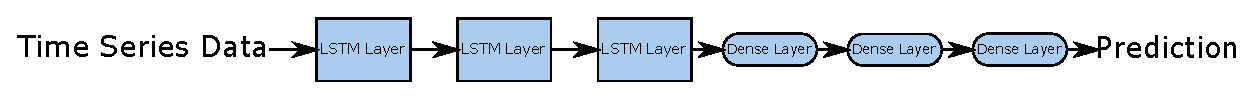
\includegraphics[width = 1 \linewidth]{model1.eps}
	\caption{Mean prediction model}
	\label{label1}
\end{figure}

\begin{figure}
	\centering
	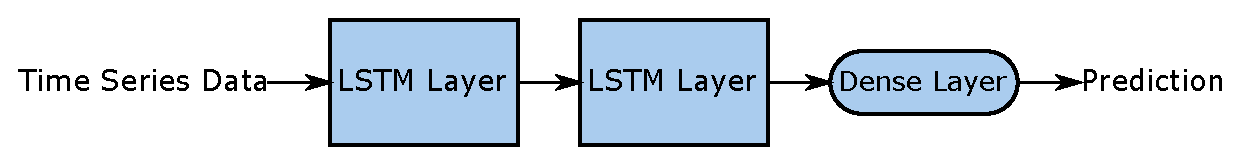
\includegraphics[width = 1 \linewidth]{model2.eps}
	\caption{Deviation from mean and deviation from median models}
	\label{label2}
\end{figure} 
 
\begin{figure}
	\centering
	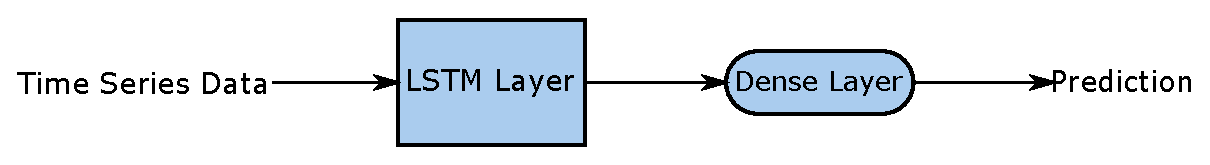
\includegraphics[width = 1 \linewidth]{model3.eps}
	\caption{Deviation from M-estimator models}
	\label{label3}
\end{figure} 

\begin{algorithm}[t]
	%
	\begin{algorithmic}[1]
		\renewcommand{\algorithmicrequire}{\textbf{Input:}}
		\renewcommand{\algorithmicensure}{\textbf{Output:}}
		\REQUIRE
		$TS$ - Time series data 
		\ENSURE
		$X$ - All outliers
		
		%
		\STATE{$TS \leftarrow$ call $Segmentation$ with $TS$}
		\STATE{$X = []$}
		\FOR{each $segment$ in $TS$}
		\FOR{each $x$ in $segment$}
		\STATE{$input \leftarrow$ middle 50\% values of $segment$}
		\STATE{$mean \leftarrow$ predict with mean LSTM model on $input$}
		\STATE{$meanDev \leftarrow$ predict with deviation from mean LSTM model on $input$}
		\STATE{$meanOutlier \leftarrow$ call $outlierTest$ with $\alpha, x, mean, meanDev$}
		\STATE{$median \leftarrow$ median of $segment$}
		\STATE{$medianDev \leftarrow$ predict with deviation from median LSTM model on $input$}
		\STATE{$medianOutlier \leftarrow$ call $outlierTest$ with $\beta, x, median, medianDev$}
		\STATE{$MEst \leftarrow$ M-estimator of $segment$}
		\STATE{$MEstDev \leftarrow$ predict with deviation from M-estimator LSTM model on $input$}
		\STATE{$MEstOutlier \leftarrow$ call $outlierTest$ with $\gamma, x, MEst, MEstDev$}
		\IF{at least two of $meanOutlier$, $medianOutlier$, and $MEstOutlier$ are \TRUE}
		\STATE{add $x$ to $X$}
		\ENDIF
		%\STATE{$isOutlier = DetectOutliers(segment, x)$}
		%\IF{$j == 0 $ \OR $ j == |segment| - 1$}
		%\IF{$isOutlier$}
		%\STATE{$truePositives += 1$}
		%\ELSE
		%\STATE{$falseNegatives += 1$}
		%\ENDIF
		%\ELSE
		%\IF{$isOutlier$}
		%\STATE{$falsePositives += 1$}
		%\ENDIF
		%\ENDIF
		\ENDFOR
		\ENDFOR
		%\STATE{$P = truePositives / (truePositives + falsePositives)$}
		%\STATE{$R = truePositives / (truePositives + falseNegatives)$}
		%\STATE{$F = \frac{2 \times P \times R}{P + R}$}
		
		%
	\end{algorithmic}
	%
	\caption{Main algorithm}
	\label{main_algorithm}
\end{algorithm}


\subsubsection{Main algorithm}To solve the problem of anomaly detection in time series data, algorithm~\ref{main_algorithm} is used. Algorithm~\ref{main_algorithm} segments the time series data and applies outlier tests on based on three test statistics exhibited in the time segments. The algorithm is illustrated in  Figure~\ref{anomalyDetectionModel}. Algorithm~\ref{main_algorithm} use algorithms~\ref{segmentation}-\ref{outlier_test} to determine which traffic flow values are outliers.
Algorithm~\ref{main_algorithm} takes time series data $TS$ as an input and returns an array $X$ containing all detected outliers.
In step 1, algorithm~\ref{main_algorithm} runs  algorithm~\ref{segmentation}. Algorithm~\ref{segmentation} divides the time series data into segments of size $K$ where each segment contains values $X_i, ... , X_{i + K}$ such that $0 \leq i \leq n - K$ and introduces outliers in each time segment. Step 2 initializes the array $X$. Steps 3-20 describe the outer loop which iterates over each time segment. Steps 4-19 describe the inner loop which iterates over all traffic flow values in the given time segment. Step 5 assigns to $input$ the middle $50\%$ slice of the time segment. Steps 6 and 7 assign to $mean$ and $meanDev$ the predicted mean and deviation from the mean using the relevant LSTM networks to predict on $input$. Step 8 conducts the statistical test for outliers using the parameters $\alpha$, $mean$, $meanDev$ and assigns a boolean value to $meanOutlier$. Step 9 assigns to $median$ the median of the time segment $segment$. Step 10 assigns to $medianDev$ the predicted deviation from the median using the relevant LSTM network to predict on $input$. Step 11 conducts the statistical test for outliers using the parameters $\beta$, $median$, $medianDev$ and assigns a boolean value to $medianOutlier$. Step 12 assigns to $MEst$ the M-esetimator of the time segment $segment$. Step 13 assigns to $MEstDev$ the deviation from the M-estimator using the relevant LSTM network to predict on $input$. Step 14 conducts the statistical test for outliers using the parameters $\gamma$, $MEst$, $MEstDev$ and assigns a boolean value to $MEstOutlier$. Step 15-16 classify outliers if at least two of our statistical tests identified the given value $x$ as an outlier. Step 13 assigns to $isOutlier$ true if at least two of $meanOutlier$, $medianOutlier$, and $MEstOutlier$ are true. Step 16 adds the value $x$ to $X$.

\begin{figure}
	\centering
	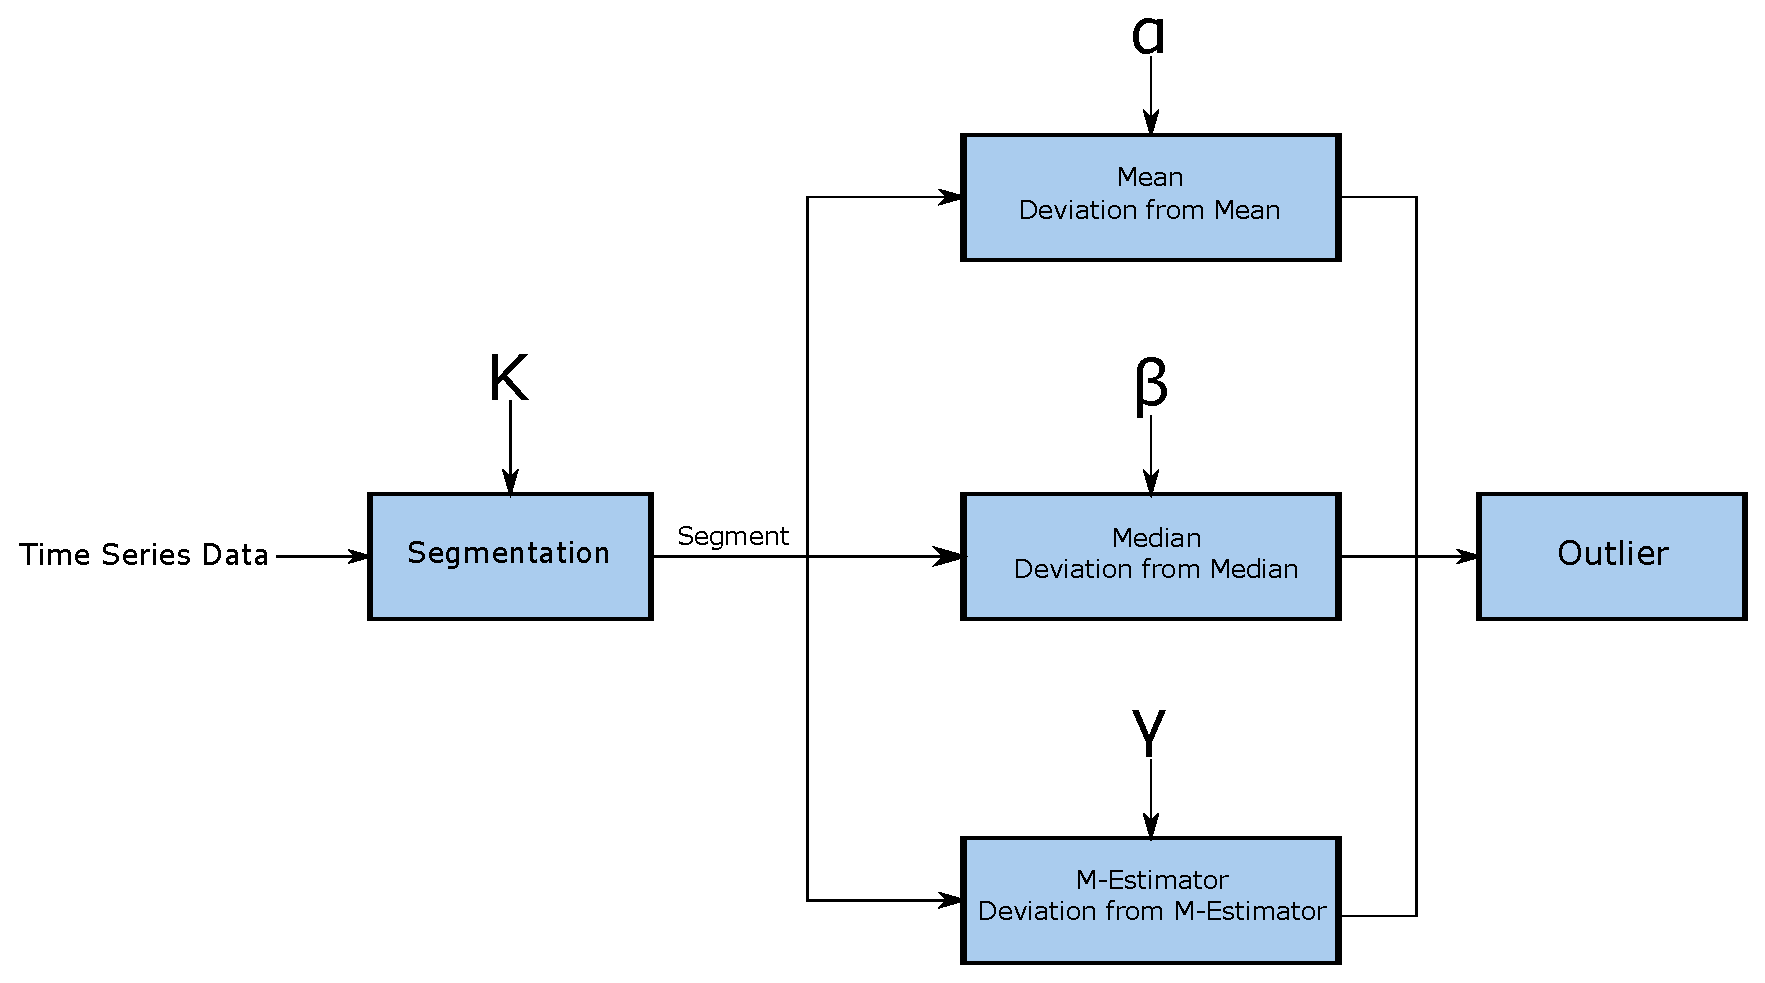
\includegraphics[width = 1 \linewidth]{anomalyDetectionModel.eps}
	\caption{Anomaly Detection Model}
	\label{anomalyDetectionModel}
\end{figure} 

\begin{algorithm}[t]
	%
	\begin{algorithmic}[1]
		\renewcommand{\algorithmicrequire}{\textbf{Input:}}
		\renewcommand{\algorithmicensure}{\textbf{Output:}}
		\REQUIRE
		$TS$ - Time series data \\
		$K$ - Segment size
		\ENSURE
		$TSNew$ - Segmented time series data with outliers
		
		%
		\STATE{$TSNew = []$}
		\FOR{$i \leftarrow 0$ \TO $|TS| - K$}
		\STATE{$segment \leftarrow TS[i:i+K]$}
		\STATE{$stddev \leftarrow deviation(segment)$}
		\STATE{$sort(segment)$}
		\STATE{$segment[0] \leftarrow segment[0] - (3*stddev)$}
		\STATE{$segment[K - 1] \leftarrow segment[K - 1] + (3*stddev)$}
		\STATE{$TSNew.append(segment)$}
		\ENDFOR
		
		%
	\end{algorithmic}
	%
	\caption{Segmentation of time series data}
	\label{segmentation}
\end{algorithm}

\subsubsection{Segmentation of time series data}Algorithm~\ref{segmentation} segments the existing time series data into segments of size $K$ and introduces outliers in each segment. Step 1 initializes the new time series array. Steps 2-9 creates $|TS| - K$ time segments. Step 3 assigns to  $segment$ values $X_i, ... , X_{i + K}$ such that $0 \leq i \leq n - K$. Step 4 calculates the standard deviation of $segment$ and step 5 sorts $segment$. Steps 6 and 7 increase the maximum value of each time segment by three standard deviations and decrease the minimum value of each time segment by three standard deviations. Step 8 adds the new time segment to $TSNew$.



%\subsubsection{Outlier detection}After the time series data has been segmented and outliers have been inserted, algorithm~\ref{outlier_detection} conducts anomaly detection by taking in the time segment $segment$ and the given traffic value $x$ as input. 

 
%\begin{algorithm}[t]
	%
%	\begin{algorithmic}[1]
%		\renewcommand{\algorithmicrequire}{\textbf{Input:}}
%		\renewcommand{\algorithmicensure}{\textbf{Output:}}
%		\REQUIRE
%		$segment$- Time segment \\
%		$x$ - Traffic flow value
%		\ENSURE
%		$isOutlier$ - Boolean value
%		
		%
%		\STATE{$fiftyPercent = |segment| / 2$}
%		\STATE{$bound = fiftyPercent / 2$}
%		\STATE{$input = segment[fiftyPercent-bound:fiftyPercent+bound]$}
%		\STATE{$mean = meanLSTM.predict(input)$}
%		\STATE{$meanDev = meanDevLSTM.predict(input)$}
%		\STATE{$meanOutlier = outlierTest(\alpha, x, mean, meanDev)$}
%		\STATE{$median = median(segment)$}
%		\STATE{$medianDev = medianDevLSTM.predict(input)$}
%		\STATE{$medianOutlier = outlierTest(\beta, x, median, medianDev)$}
%		\STATE{$MEst = MEstimator(segment)$}
%		\STATE{$MEstDev = MEstDevLSTM.predict(input)$}
%		\STATE{$MEstOutlier = outlierTest(\gamma, x, MEst, MEstDev)$}
%		\STATE{$isOutlier = meanOutlier$ \AND $(medianOutlier$ \OR $MEstOutlier)$ \OR $(medianOutlier$ \AND $MEstOutlier)$}
		%
%	\end{algorithmic}
	%
%	\caption{Outlier detection}
%	\label{outlier_detection}
%\end{algorithm}


\begin{algorithm}
	%
	\begin{algorithmic}[1]
		\renewcommand{\algorithmicrequire}{\textbf{Input:}}
		\renewcommand{\algorithmicensure}{\textbf{Output:}}
		\REQUIRE
		$param$ - Tunable parameter \\
		$x$ - Traffic flow value \\
		$m$ - Test statistic \\
		$dm$ - Deviation from test statistic
		\ENSURE
		$isOutlier$ - Boolean value
		
		%
		\STATE{$isOutlier \leftarrow (m - param * dm > x)$ \OR $(m + param * dm < x)$}
		%
	\end{algorithmic}
	%
	\caption{Outlier test}
	\label{outlier_test}
\end{algorithm}

\subsubsection{Outlier test}Algorithm~\ref{outlier_test} describes the statistical test in which the test statistics are used to classify a value as an outlier. Algorithm~\ref{outlier_test} takes a tunable parameter $param$, a traffic flow value $x$, a test statistic $m$, and the deviation from the test statistic $dm$ as input. In step 1, the algorithm assigns to $isOutlier$ the boolean result of $x > m + \alpha * dm$ or $x < m - \alpha * dm$. This calculates if the given $x$ is greater than the upper bound of the statistical test or if $x$ is lower than the lower bound of the statistical test. If so, it is an outlier.
   

%
%================================================================%
%                        RESULTS
%================================================================%
%
\section{Results}
\label{results}
We computed Precision, Recall, and F-measure to assess the effectiveness of our anomaly detection model on traffic series data with outliers inserted in each segment. With a segment size $K = 12$, we measured the changes in Precision, Recall, and F-measure by keeping two tunable parameters constant while varying the third. We varied the third tunable parameter in increments of $0.25$ from $0.5$ to $4.25$ while keeping the other two tunable parameters fixed at $2.0$.

\subsection{Analysis of Parameter Variation} Figure~\ref{alphaResults} shows the changes in the statistical metrics when the parameter $\alpha$, corresponding to the outlier test using the mean, is changed. As shown in the figure, even when the $\alpha$ parameter is low, i.e. the outlier test threshold is highly sensitive, we are able to measure a very high rate of effectiveness with our algorithm, with Precision over $90\%$ and Recall over $80\%$. Note that as $\alpha$ increases, there is an inverse correlation between Precision and Recall. This is to be expected as the threshold of outlier classification using the mean becomes higher. Innocuous values are less likely to be classified, leading to fewer false positives, but outlier values are less likely to lie outside the outlier test threshold, leading to more false negatives. The best balance between Precision and Recall appears to be when $\alpha = 0.5$, as the F-measure value is the highest at that point.

Figure~\ref{betaResults} shows the changes in statistical metrics when the parameter $\beta$, corresponding to the outlier test using the median, is changed. As shown in the figure, we again observe an inverse correlation between Precision and Recall, with Recall being higher at low values of $\beta$ and Precision being higher at high values of $\beta$. These changes are much more precipitous than that of the $\alpha$ parameter. Interestingly, Precision appears to decline slightly at high values of $\beta$. The best balance between Precision and Recall appears to be at $\beta = 1.5$, where the F-measure is highest.

Figure~\ref{gammaResults} shows the changes in statistical metrics when the parameter $\gamma$, corresponding to the outlier test using the M-estimator, is changed. We again observe the inverse correlation between Precision and Recall. However, the rate of increase of Precision is much greater than the rate of decrease of Recall than observed in the $\alpha$ and $\beta$ metrics. As a result, we observe the highest F-measure value at $\gamma = 2.25$, higher than that of the previous two parameters.

\begin{figure}
	\centering
	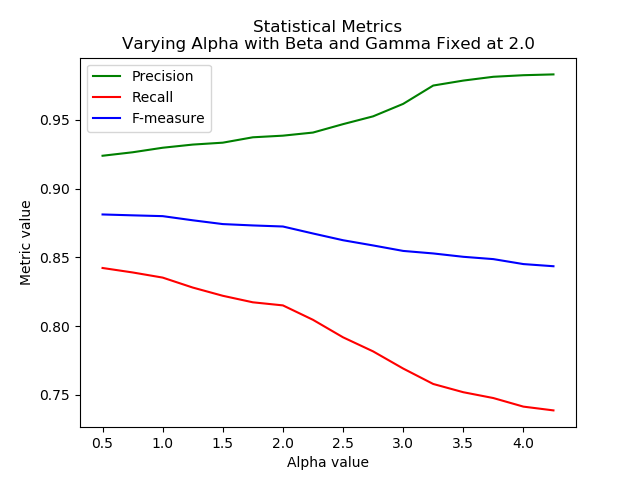
\includegraphics[width = 0.95 \linewidth]{AlphaResults.png}
	\caption{Metric Changes When Alpha is Varied}
	\label{alphaResults}
\end{figure}
\begin{figure}
	\centering
	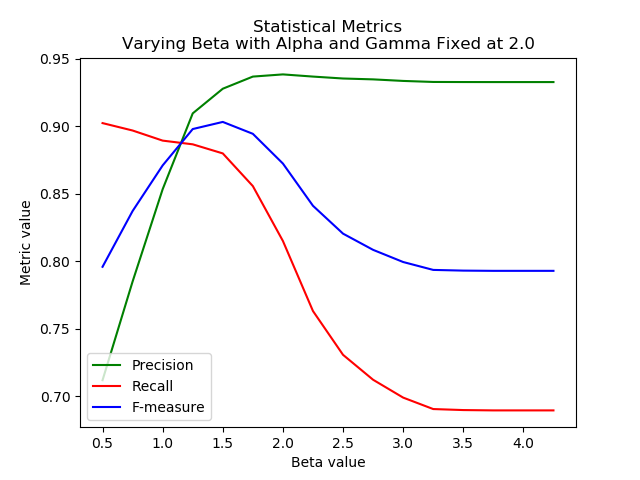
\includegraphics[width = 0.95 \linewidth]{BetaResults.png}
	\caption{Metric Changes When Beta is Varied}
	\label{betaResults}
\end{figure}
\begin{figure}
	\centering
	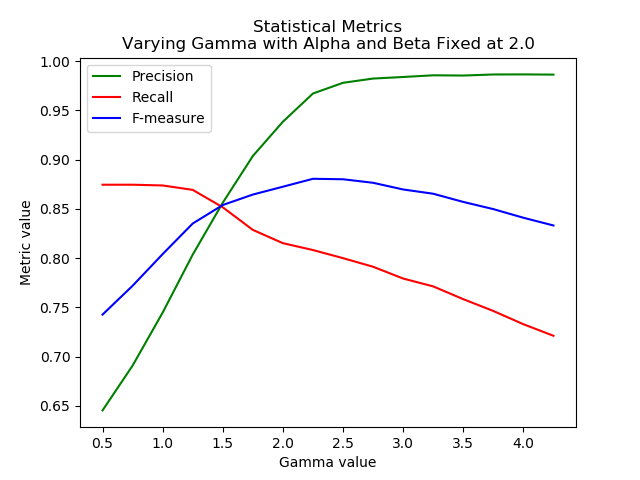
\includegraphics[width = 0.95 \linewidth]{GammaResults.png}
	\caption{Metric Changes When Gamma is Varied}
	\label{gammaResults}
\end{figure}

\subsection{Analysis of Outlier Magnitude}
The table below illustrates the changes in each of the Precision, Recall, and F-measure metrics when the outliers of each segment are modified by a value of the given magnitude times the standard deviation of the time segment. By Algorithm~\ref{segmentation}, we generate two outliers, high and low, in each segment by modifying them by $3$ standard deviations. We measured the Precision, Recall, and F-measure values when the outlier magnitude was varied from $1-10$ rather than fixed at a default value of $3$. We observed that Precision and tended to increase as magnitude increases. We also observed that Recall also tended to increase, but it appeared to level out at around $0.83-0.84$. Both results are to be expected as the outlier test becomes less sensitive to outliers as magnitude increases, and we see more true positives and fewer false positives. Interestingly, Recall appears to decrease at higher values of magnitude. This may be due to the variability in outliers being on the threshold of the outlier tests.

\begin{center}
	\begin{tabular}{|c|c|c|c|}
		\hline
		Magnitude & Precision & Recall & F-measure \\
		\hline
		1 & 0.78044 & 0.74676 & 0.76323 \\
		\hline
		2 & 0.88451 & 0.80065 & 0.84049 \\
		\hline
		3 & 0.93852 & 0.81512 & 0.87248 \\
		\hline
		4 & 0.97286 & 0.82285 & 0.89159 \\
		\hline
		5 & 0.98755 & 0.83134 & 0.90274 \\
		\hline
		6 & 0.99351 & 0.84007 & 0.91037 \\
		\hline
		7 & 0.99676 & 0.84356 & 0.91378 \\
		\hline
		8 & 0.99882 & 0.84132 & 0.91333 \\
		\hline
		9 & 0.99970 & 0.83683 & 0.91104 \\
		\hline
		10 & 1.0 & 0.83383 & 0.90938 \\
		\hline
	\end{tabular}
\end{center}

\subsection{Analysis of Outlier Percentage}
The table below illustrates the changes in each of the Precision, Recall, and F-measure metrics when the percentage of outliers are modified in each time segment. With a segment size $K = 12$ and assuming that the middle $50\%$ values are not outliers, we measure the Precision, Recall, and F-measure values when the outlier percentage is varied from $0-50\%$, or when there are $0-6$ outliers in each segment. We observed that Precision tended to increase until it reached its highest value at $16.667\%$, or when there were two outliers in each time segment. Afterwards, we observed a decrease in Precision. We also observed that Recall was between $0.45$ and $0.5$ at low outlier percentages, but leveled out at around $0.815$ when there were two or more outliers in the time segment. Our algorithm appears to be most effective when there are few, yet not many outliers in the time series data.

\begin{center}
	\begin{tabular}{|c|c|c|c|}
		\hline
		Percentage & Precision & Recall & F-measure \\
		\hline
		0 & 0.60992 & 0.46657 & 0.52870 \\
		\hline
		8.3333 & 0.89986 & 0.49326 & 0.63723 \\
		\hline
		16.667 & 0.93852 & 0.81512 & 0.87248 \\
		\hline
		25 & 0.66355 & 0.81437 & 0.73126 \\
		\hline
		33.333 & 0.51719 & 0.81462 & 0.63269 \\
		\hline
		41.667 & 0.42528 & 0.81587 & 0.55912 \\
		\hline
		50 & 0.36018 & 0.81562 & 0.49969 \\
		\hline
	\end{tabular}
\end{center}

\section{Conclusions}
\label{conclusion}
This paper highlights the challenges behind anomaly detection as it relates to large quantities of time series data. We presented an automated anomaly detection algorithm that relies on supervised learning and statistical methods to determine outliers within the time series. Our proposed anomaly detection algorithm relies on segmentation to determine outliers within their local contexts. We measured the efficacy of our algorithm from different perspectives, namely variation in tunable parameters, outlier magnitude, and outlier quantity, and quantified it in terms of Precision, Recall, and F-measure in each case. Our algorithm does best with smaller tunable parameter values with low yet not insignificant amounts of outliers.



%\section*{Acknowledgement}
%This research is supported by NSF CAREER grant CNS \#1346600.

%\nocite{pppOCWCTSGA10}
%
%================================================================%
%                        REFERENCES
%================================================================%
%
{
	\bibliographystyle{IEEEtran}
	\bibliography{IEEEabrv,ResourceSharing}
}
%


\end{document}
}
	content
\end{environment-name}